\documentclass[conference]{../cls/IEEEtran}

\usepackage{graphicx}

\begin{document}

\title{Early Estimation of Multi-Objective Traffic Behavior}

\author{
	\IEEEauthorblockN{Dominik Ascher}
	\IEEEauthorblockA{
		Chair IV: Software \& Systems Engineering\\
		Technische Universit\"at M\"unchen\\
		Boltzmannstr.\ 3, 85748 Garching, Germany\\
		Email: ds.ascher@gmail.com
	}
	\and
	\IEEEauthorblockN{Georg Hackenberg}
	\IEEEauthorblockA{
		Chair IV: Software \& Systems Engineering\\
		Technische Universit\"at M\"unchen\\
		Boltzmannstr.\ 3, 85748 Garching, Germany\\
		Email: hackenbe@in.tum.de
	}
}

\maketitle

\begin{abstract}
Intelligent Transportation Systems (ITS) have come a long way targeting recent problems of increasing emissions and growing vehicle numbers. Current approaches address a variety of objectives including congestion management, collision avoidance, energy-efficiency and emission reduction. However, respective solutions typically are designed for and tailored to a fixed subset of objectives. Consequently, the effects of changing objectives and priorities cannot be assessed easily. To overcome this situation we present a lightweight approach to estimating traffic behavior early in the systems engineering process using discrete-time and continuous-state system models. We demonstrate the feasibility of the framework using a basic traffic scenario before closing with a first conclusion and outlook.
\end{abstract}

\begin{IEEEkeywords}
Feasibility study, intelligent transportation systems.
\end{IEEEkeywords}

\section{Motivation}
\label{sec:motivation}

In recent decades, efforts to engineer ITS have come a long way, targeting contemporary and future problems of increasing emissions and growing vehicle numbers. Among the approaches two main directions can be distinguished: (1) Urban Traffic Control (UTC) focusing on multiple traffic participants and their interaction~\cite{Chen2010,Dresner2008} and (2) Eco-Routing focusing on a single traffic participant and his route~\cite{Ericsson2006,Boriboonsomsin2012}. In particular, UTC typically targets congestion management and collision avoidance~\cite{Chen2010}. Technically, the approaches rely on agent based techniques to describe human driving behavior with respect to traffic supervision and control~\cite{Chen2010}. More advanced approaches even consider fully autonomous vehicles thereby proposing an alternative to human-oriented traffic supervision and control~\cite{Dresner2008}. In contrast, Eco-Routing typically targets energy-efficiency and emission reduction~\cite{Ericsson2006}. Technically, the approaches rely on optimization techniques to describe route variables, constraints and objectives~\cite{Ericsson2006}. As frequent use of energy-efficient routes might cause congestion, advanced approaches finally incorporate historical and real-time traffic information thereby taking first steps towards bridging the gap between Eco-Routing and UTC~\cite{Boriboonsomsin2012}. Common among all previous approaches are objectives like congestion management, collision avoidance, energy-efficiency and emission reduction.

However, while the presented approaches offer tailored solutions for a fixed set of objectives, they are not designed to estimate the effect of changing objectives and priorities. In particular, it is important to estimate this effect in early phases of systems engineering (such as requirements discovery or feasibility study) to uncover potential opportunities and threats~\cite{Whitten2005}. To overcome this situation in the following we present a lightweight model-based approach.

\section{A Lightweight Model-Based Approach}
\label{sec:approach}

An overview of our model-based approach to traffic behavior estimation is shown in Figure~\ref{fig:framework}. Technically, we base our work on emergent property estimation techniques described in~\cite{Hackenberg2012}. Consequently, we use a discrete-time and continuous-state system model. We rely on discrete-time models to reduce the reachable state space during behavior estimation. However, we work with continuous-state models because quantities like velocity or distance can be described more intuitively. Further, we employ a generic model architecture separating between context, constraint, objective, software and equivalence model. The non-deterministic software model describes the optimizable control behavior (not the control logic), while the context model describes the controlled physical state. Based on the physical state the constraint and objective models define the operational limits and costs. Finally, the equivalence model describes how the physical states can be clustered during optimization. For control behavior estimation the framework finally integrates stochastic approximation techniques~\cite{Pereira1991} to achieve robustness against arbitrary cost functions.

\begin{figure}[h]
	\centering
	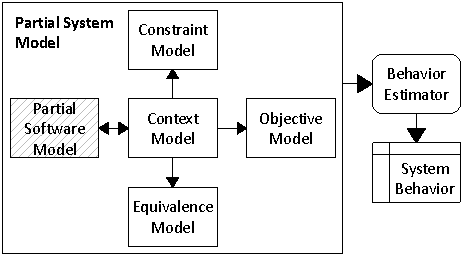
\includegraphics{../gfx/framework.pdf}
	\caption{Overview of the model-based approach to traffic behavior estimation.}
	\label{fig:framework}
\end{figure}

The approach is similar to work on vehicle path optimization~\cite{Danielsson2007}, which uses Modelica to specify dynamic optimization problems and Optimica for out-of-the-box optimization. However, the authors use continuous-time models and concentrate on single vehicles only.

\section{Its Application to Traffic Systems}

In the following we apply the approach to a basic traffic scenario including various participants as well as common time and energy objectives.

\subsubsection*{Model}

To reduce the physical state space for behavior estimation, in our model the traffic infrastructure is represented as directed graph consisting of nodes and edges. Nodes constitute reference points in the environment such as junctions and are defined by their absolute position, i.e.\ latitude, longitude and elevation. Edges represent road segments and are defined by source and target node as well as assigned number of lanes. Finally, for demonstration we use a time resolution of 60 seconds, but other resolutions are supported as well.

The \textit{context model} is composed of vehicle components, which define several inputs and outputs for each time step: Inputs are the speed and the target position (i.e.\ edge) on the traffic infrastructure represeting a routing decision in case a node is passed. Outputs again are the position, the distance travelled on the edge, the energy consumption and the state of charge. The energy consumption is estimated from the travelled elevation profile and the speed. Based on the vehicle positions (i.e.\ edges) and travelled distances on the edges the \textit{constraint model} tests for collisions. Collisions occur in case the number of vehicles intersecting on the same edge exceeds the number of assigned lanes. Note that the constraint does not consider the intermediate driving behavior between two time points. This simplification was chosen since we are not interested in such microscopic effects. Then, the \textit{objective model} encodes two conflicting objectives: Energy-efficiency and shortest travelling time. Both system-level objectives are decomposed into equivalent vehicle objectives. Per vehicle energy-efficiency is measured in terms of cummulative energy consumption needed while traveling from origin to destination. In contrast shortest traveling time is measured in terms of time steps needed while traveling from origin to destination. At system-level the independent vehicle objectives are aggregated using respective weights for energy-efficiency and shortest traveling time. To complete the control loop the \textit{software model} encodes non-deterministic selection of speed and target position per vehicle. The speed interval is discretized uniformly into a constant number of steps. In contrast, the target position is obtained from the set of outgoing edges of the target node of the curre position. Finally, the \textit{equivalence model} uses the average state of charge over all vehicles for clustering the state space. This rule has been selected after testing several clustering strategies.

\subsubsection*{Analysis}

For evaluating our approach, we describe a basic traffic scenario including multiple vehicles: Each vehicle uses the same origin and destination. There are two different routes to drive from origin to destination. The first route represents a longer, but flat route, while the second route describes a shorter, but undulating route. To demonstrate behavior estimation, we analyze two weight configurations of the energy and time objectives. Configuration A favors lower energy consumption, while configuration B favors shorter travel time.

An estimation for the resulting traffic behavior of the two
configurations is depicted in Figure 2, showing the vehicles route selection
and aggregated energy consumption over time. Configuration A shows
stronger vehicle affinity to more energy-efficient (flat) route selection and
less energy consumption in comparison to configuration B. Configuration B exerts
vehicle affinity towards shortest route selection, causing increased energy
consumption, but results in less elapsed time in comparison to configuration A.
In addition to the assigned weighting of objectives in both configurations,
congestion within the traffic system has possibly influenced vehicle
route selection and energy consumption as observed vehicle behavior deviated
from expected vehicle behavior in regard to respective objective weighting.

\begin{figure}[t!]
	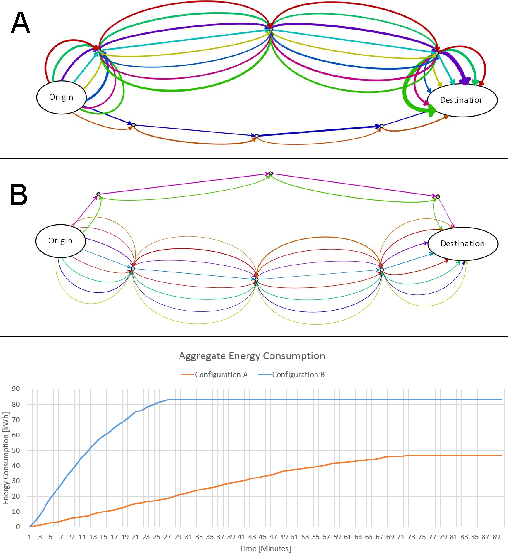
\includegraphics[width=\columnwidth]{../gfx/results.pdf}
	\caption{Comparison of routes (top) and aggregate energy consumption
	(bottom) for weight preference  on (A) energy-efficient and (B) time.}
	\label{figure:results}
\end{figure}

\section{Conclusion and Outlook}

The preliminary results are encouraging with respect to the feasibility of the model-based approach for multi-objective behavior estimation in the domain of traffic systems. Currently, we are working on a detailed model description, a larger-scale demonstrator, more diverse objectives and the inclusion of multi-modal travelling facilities such as bicycles and trains.

\bibliographystyle{../bst/IEEEtran}
\bibliography{ICCVE-2014}

\end{document}
